\chapter{Simple quantum systems}

In this chapter, we will review some technique and materials 
for you to implement quantum simulation with quantum computer.
Formulation of the system and requirements and progress are discussed 
in the below sections.
The contents are dicussed in aiming a specific quantum systems,
1 dimensional particle systems.
It is a very classical example of the physics system but
has many attributes to study in quantum mechanics.

\textbf{Note}: It is not a full coverage of the quantum simulation with 
quantum computer. There are plenty of different quantum systems and 
they need individual modeling techniques.


\section{Modeling of 1dim Particle}
\label{sec:simulation}

Now let's take an example, this was introduced in \textit{Box 4.12} in Nielsen and Chuang textbook. 
The particle in 1-dim system of momentum and mass, $p, m$ and the potential, $V$ can be expressed with next hamiltonian.

\begin{equation}
    \mathcal{H} = \frac{p^2}{2 m} + V
\end{equation}

The wave function of the system is $| \psi \rangle$. 
If we discretize the line with $n$ number of subregions, $x_1, x_2, \dots x_n$, 
wave function have next representations.

\begin{align}
    | \psi _d \rangle =& \int_{-\infty}^\infty |x \rangle \langle x| | \psi \rangle \, dx \\
                      =& \int_{-L}^L |x \rangle \langle x| | \psi \rangle \, dx \\
                      \approx& \sum \lambda_i | x_i \rangle
\end{align}

The last representation is a finite approximation of the quantum system.
Using computation basis and their binary representation, where $0111 = 1*2^0 + 1*2^1 + 1*2^2 + 0*2^3 = 7$,
we can simulate the $-d \leq x \leq d$ region particle wave function with 

\begin{equation}
    |\psi \rangle = \sum_{k = - d/\Delta x}^{d/{\Delta x}} \lambda_k | k \Delta x \rangle 
\end{equation}

The expectation value of the position is measured with the observable, $\mathbf{X}$

\begin{equation}
    \mathbf{X} = \sum i \Delta x |i \Delta x  \rangle \langle i \Delta x |
\end{equation}

\begin{equation}
    \langle x \rangle = \langle \psi_d |\mathbf{X} | \psi_d \rangle
\end{equation}


Similarly, the momentum observable is 

\begin{equation}
    \mathbf{P} = \sum_{j} p_j |k_j  \rangle \langle k_j |
\end{equation}



In the representation the $V$ term can be expressed with $x_i$ operators directly, however if some 
observables are defined with $\hat{p}$, we needs a transformation. 
In continuous space, the canonical variables have next relationship on Fourier transformation.

\begin{eqnarray}
    \phi(p) &=& \frac{1}{\sqrt{2\pi \hbar}}\int \psi(x) \exp\left(- i \frac{px}{\hbar} \right) \, dx \\
    \psi(x) &=& \frac{1}{\sqrt{2\pi \hbar}}\int \phi(p) \exp\left( i \frac{px}{\hbar} \right) \, dp 
\end{eqnarray}

In matrix representation,

\begin{eqnarray}
    H &=& \sum_{ij} h_{ij} | x_j \rangle \langle x_i| \\
      &=& P + V \\
      &=& (\mbox{QFT})(\sum_{i} p_{i} | p_i \rangle \langle p_i|) (\mbox{QFT}^{\dagger}) + \sum_{ij} v_{ij} | x_j \rangle \langle x_i|
\end{eqnarray}

where, $\mbox{QFT}$ is a quantum fourier transform. 

\begin{figure}[ht]
    \begin{tikzpicture}
        A
    \end{tikzpicture}
\end{figure}

We can discrete the wave function as $n$ number of discreted vector, $\{|x_i \rangle \}_{n}$ indicating the probability of finding the particle in $x_i \pm \Delta x$ region.
With manuplating $V$ value by the time, we can simulate various experiment, such as slit experiment or quantum tunneling effects.
See section \ref{sec:simulation} for details of implementation.


One thing you can confuse in the above matrx representation is canonical commutation relationship. 

\begin{equation}
    [\hat{x}, \hat{p}] = i \hbar
\end{equation}

Now the observables are indicated in finite dimension matries,  $\mathbf{X}, \mathbf{P}$. 
They would be diagonal matrix in each basis. Question is that "Is the canonical commutation relationship preserved in 
the matrix representation?" Unfortunately, the answer is \textbf{no}.
You may think that it is because of the low precision of discrete Fourier transformation in finite dimension.
It could be a reason, then how much precision is required to meet the $[\hat{x}, \hat{p}] = i \hbar$?  
The answer is $\infty$. The fact is that the operator $\hat{x}$ and $\hat{p}$ are not bounded operators. 

We can prove the unboundness of the operators, easily.
\begin{align*}
    [\hat{x}^n, \hat{p}] = i \hbar n \hat{x}^{n-1}\\
    2 ||\hat{p}|| || \hat{x}||^n \geq || \hat{x}^n \hat{p} || + || \hat{p} \hat{x}^n || \geq n \hbar ||\hat{x}||^{n-1}\\
    2 ||\hat{x}|| ||\hat{p}|| \geq n \hbar
\end{align*}

the above inequality hold for \textbf{any} $n\geq 1$. 

In fact, in the finite dimension, the canonical relationship should be $[\hat{x}, \hat{p}] = 0$,
only if in the infinite dimension, $[\hat{x}, \hat{p}] = 1$ and if we approximate $n\rightarrow \infty$ 
the commutator $[\hat{x}, \hat{p}]$ would show Dirac-Delta like behavior\cite{santhanam_quantum_1976}.

\subsection{Modeling a Hamiltonian}

One thing you kepp in mind is that 
the finite dimension modeling with Weyl's clock and shift method.
The position domain is not a straight long 1 dimension line.
It would be a circular loop position, where $|2^n \rangle= |0 \rangle$.
Some 1 dim simulation have those error, especially, when they simulate 
the quantum tunneling. 
They did not considering the circular connected space and 
mis interpretated the amplitude of wave function. %cite the

The Fig \ref{fig:quantum_tunneling_simulation}, \ref{fig:quantum_tunneling_simulation2} would be helpful understand the situation.

\begin{figure}
    \centering
    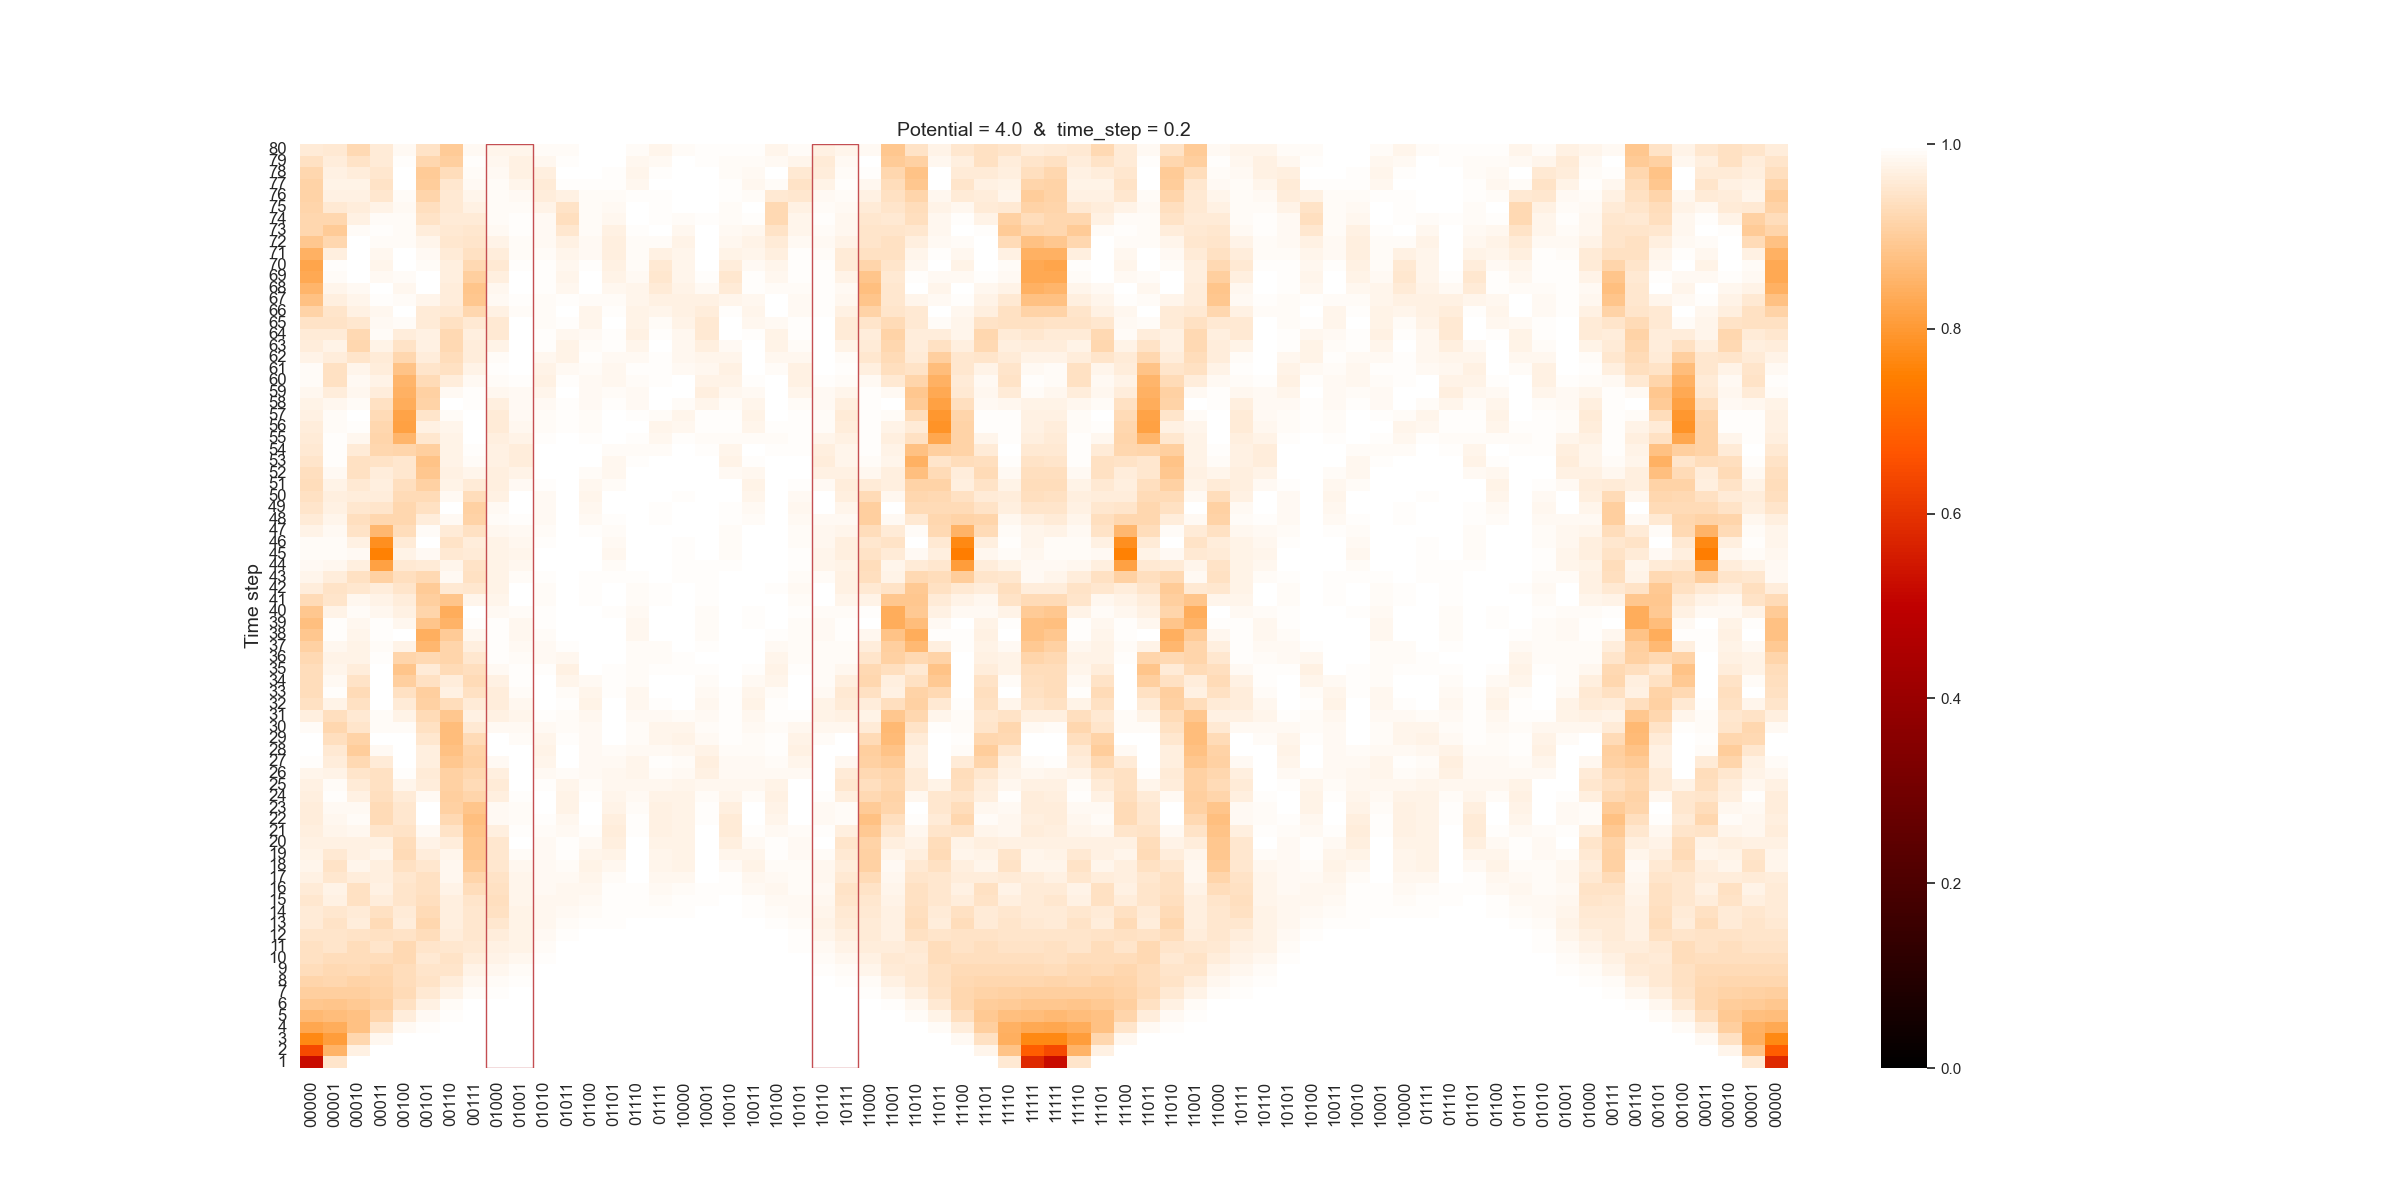
\includegraphics[width=0.95\textwidth]{media/sym_8_v_4.0.png}
    \caption{
        The symmetric potential. }
    \label{fig:quantum_tunneling_simulation}
\end{figure}

\begin{figure}
    \centering
    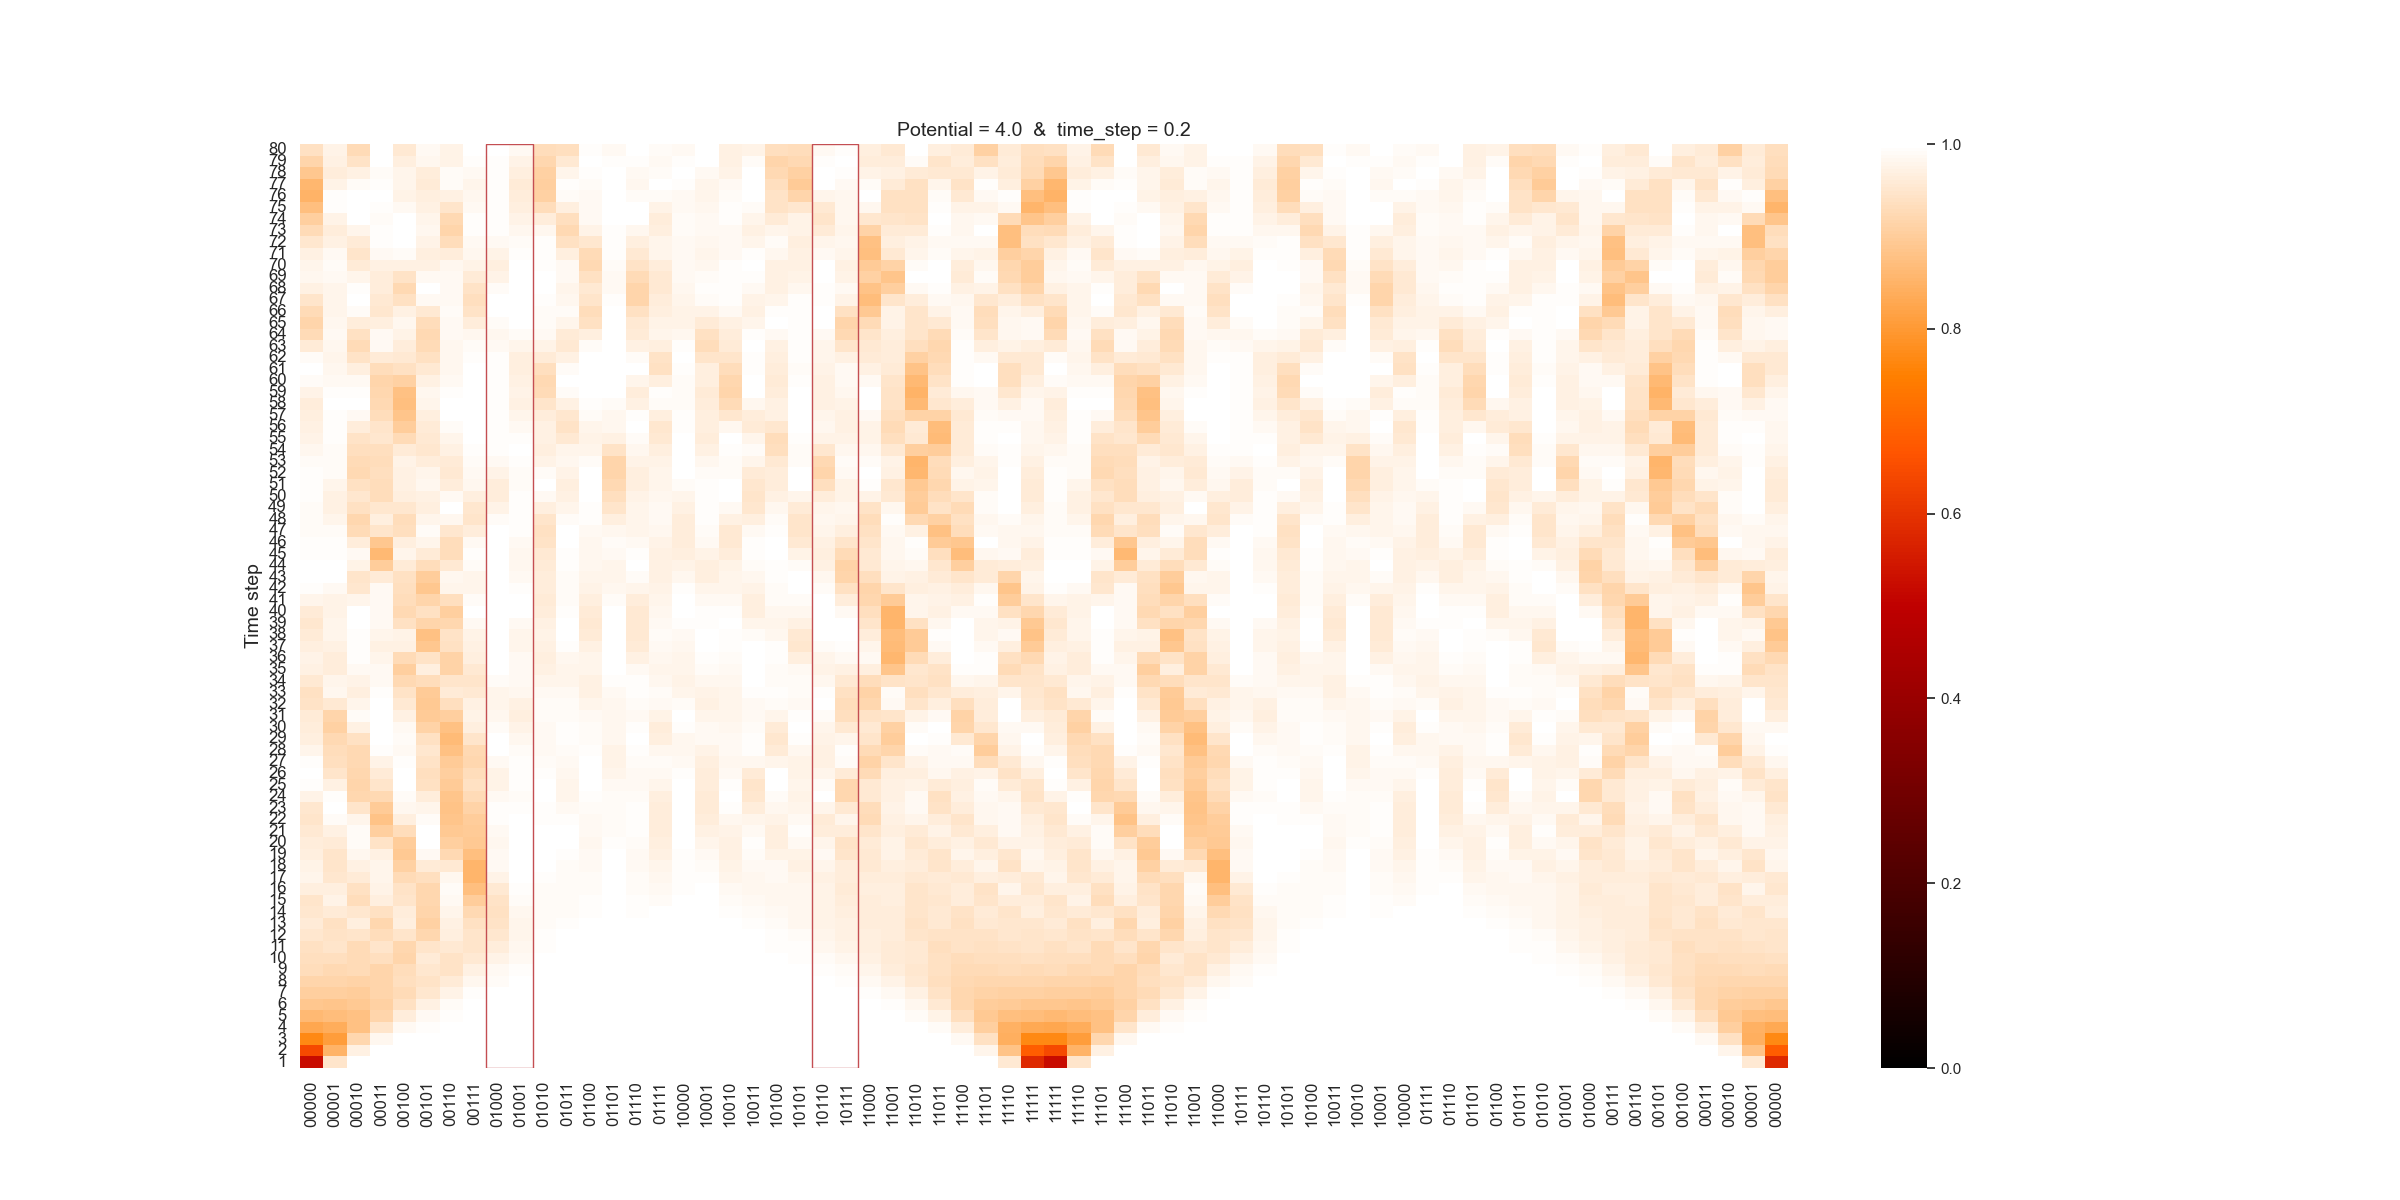
\includegraphics[width=0.95\textwidth]{media/asym_8_v_4.0.png}
    \caption{
        The reduced the right potential as $1/4$ times of the left potential.}
    \label{fig:quantum_tunneling_simulation2}
\end{figure}

\subsection{Slite experiment}
Using a tunneling circuit and 
the time dependent Hamiltonian, the Slit experiment 
could be simulated with  quantum computer where the time $t$ 
indicate the position $x$, the axis where particle is moving.
\subsection{}
